\section{Tarea}

\subsection{Objetivo}

\begin{itemize}
    \item Programar paralelamente usando treads.  
    \item Comparar los lenguajes de programación: Java, C++ y Go.
\end{itemize}



\subsection{Problema propuesto: }

\begin{enumerate}[label={ }]
    \item Sea un función cualquier, por ejemplo: f(x) = 2x
    \item 2+3x +1⁄2
    \item y los puntos a=2 y b=20
\end{enumerate}
Hallar el área bajo la curva en el primer cuadrante, utilizando el método del trapecio.
En Clase:
\begin{itemize}
    \item Utilice Java para resolver el problema.
    \item Utilice C++ para gestionar la memoria dinámicamente.
\end{itemize}
La proxima clase:
\begin{itemize}
    \item Utilice Go para resolver el problema.
\end{itemize}



\section{Equipos, materiales y temas utilizados}

\begin{itemize}
    \item Subsistema de Windows para Linux (WSL) con Ubuntu (versión predeterminada instalada mediante Microsoft Store).
    \item Sistema operativo: Microsoft Windows [Versión 10.0.26100.6584]
    %\item MiKTeX-pdfTeX 4.15 (MiKTeX 23.4) \LaTeX.
    %\item Strawberry Perl (requerido por MiKTeX para la ejecución de scripts auxiliares en la compilación de ciertos paquetes).
    \item Helix 25.01.1 (e7ac2fcd)
    \item Visual Studio Code 1.104.0 x64
    \item Git version 2.41.0.windows.1
    \item Cuenta activa en GitHub para la gestión de repositorios remotos.
    \item POO.
    \item Lenguaje de programación Java.
    \item Lenguaje de programación golang
    \item Lenguaje de programación c++
\end{itemize}




\section{URL de Repositorio Github}

\begin{itemize}
    \item URL del Repositorio GitHub para clonar o recuperar.
    \item \url{https://github.com/yhuayhuahi/Teo.git}
    \item \url{https://github.com/avillaq/Teo.git}
    \item URL para el laboratorio (\itemPracticeNumber) en el Repositorio GitHub.
    \item \url{https://github.com/yhuayhuahi/Teo/tree/main/laboratorios/lab\itemPracticeNumber}
    \item \url{https://github.com/avillaq/teo/tree/main/lab03}
\end{itemize}




\section{Desarrollo de las actividades}

\subsection {Actividades}

\subsubsection {Función Main en C++ - Primera implementación}

A continución se muestra la función principal en c++ de la primera implementación [un hilo por trapecio a generar]:

\begin{lstlisting}[style=cpp-style, caption={Función Main en cpp - Primera implementación}]
    int main() {
        cout << "---------- CALCULADORA DE INTEGRALES CON HILOS NORMALES ----------" << endl;
        cout << endl;
        
        cout << "Ingrese la función f(x) a integrar:" << endl;
        cout << "   Ejemplos:" << endl;
        cout << "   - 2*x^2 + 3*x + 0.5" << endl;
        cout << "   - sin(x)" << endl;
        cout << "   - cos(x) + x^2" << endl;
        cout << "   - exp(x)" << endl;
        cout << "   - log(x)" << endl;
        cout << "   - sqrt(x)" << endl;
        cout << endl;
        cout << "f(x) = ";
        
        getline(cin, funcion_matematica);
        
        // eliminar espacios en blanco al inicio y final
        size_t start = funcion_matematica.find_first_not_of(" \t");
        if (start == string::npos) {
            cout << "Error: No se ingreso ninguna funcion" << endl;
            return 1;
        }
        size_t end = funcion_matematica.find_last_not_of(" \t");
        funcion_matematica = funcion_matematica.substr(start, end - start + 1);
    
        cout << "Funcion ingresada: '" << funcion_matematica << "'" << endl;
    
        // validamos la funcion 
        try {
            double test1 = evaluarFuncion(funcion_matematica, 1.0);
            double test2 = evaluarFuncion(funcion_matematica, 2.0);
            if (test1 != 0.0 || test2 != 0.0) {
                cout << "Funcion valida" << endl;
            }
        } catch (...) {
            cout << "Error: La funcion no es valida" << endl;
            exit(1);
        }
        
        // se piden los parametros de la integral
        double limite_inferior, limite_superior;
        int decimales, numero_hilos;
        
        cout << "Limite inferior (a): ";
        cin >> limite_inferior;
        cout << "Limite superior (b): ";
        cin >> limite_superior;
        cout << "Numero de hilos (trapecios): ";
        cin >> numero_hilos;
        cout << "Decimales en el resultado: ";
        cin >> decimales;
        cout << endl;
        
        // validaciones
        if (limite_superior <= limite_inferior) {
            cout << "Error: El limite superior debe ser mayor al inferior" << endl;
            return 1;
        }
        
        if (numero_hilos <= 0) {
            cout << "Error: El numero de hilos debe ser positivo" << endl;
            return 1;
        }
        
        if (numero_hilos > 1000) {
            cout << "Error: Muchos hilos pueden afectar el rendimiento" << endl;
        }
    
        if (decimales < 0 || decimales > 10) {
            cout << "Error: El numero de decimales debe estar entre 0 y 10" << endl;
            return 1;
        }
        
        cout << "Iniciando calculo..." << endl;
        
        // se crean y lanzan hilos
        vector<thread> hilos;
        hilos.reserve(numero_hilos);
        
        for (int i = 0; i < numero_hilos; i++) {
            hilos.emplace_back(calcularTrapecio, limite_inferior, limite_superior, i, numero_hilos);
        }
        
        // se espera a que terminen todos los hilos
        for (auto& hilo : hilos) {
            hilo.join();
        }
    
        cout << endl;
        cout << "RESULTADO FINAL:" << endl;
        cout << "   Area = " << area_total << endl;
        cout << endl;
        
        return 0;
    }
\end{lstlisting}


\subsubsection {Función Main en C++ - Implementación con Pool}

A continución se muestra la función principal en c++ implementado con Pool de threads [un hilo para un grupo de trapecios a generar]:

\begin{lstlisting}[style=cpp-style, caption={Función Main en TrapecioPool.cpp }]
    int main() {
        cout << "---------- CALCULADORA DE INTEGRALES CON POOL DE HILOS ----------" << endl;
        cout << endl;
        
        cout << "Ingrese la función f(x) a integrar:" << endl;
        cout << "   Ejemplos:" << endl;
        cout << "   - 2*x^2 + 3*x + 0.5" << endl;
        cout << "   - sin(x)" << endl;
        cout << "   - cos(x) + x^2" << endl;
        cout << "   - exp(x)" << endl;
        cout << "   - log(x)" << endl;
        cout << "   - sqrt(x)" << endl;
        cout << endl;
        cout << "f(x) = ";
        
        getline(cin, funcion_matematica);
        
        // eliminar espacios en blanco al inicio y final
        size_t start = funcion_matematica.find_first_not_of(" \t");
        if (start == string::npos) {
            cout << "Error: No se ingreso ninguna funcion" << endl;
            return 1;
        }
        size_t end = funcion_matematica.find_last_not_of(" \t");
        funcion_matematica = funcion_matematica.substr(start, end - start + 1);
    
        cout << "Funcion ingresada: '" << funcion_matematica << "'" << endl;
    
        // validamos la funcion 
        try {
            double test1 = evaluarFuncion(funcion_matematica, 1.0);
            double test2 = evaluarFuncion(funcion_matematica, 2.0);
            if (test1 != 0.0 || test2 != 0.0) {
                cout << "Funcion valida" << endl;
            }
        } catch (...) {
            cout << "Error: La funcion no es valida" << endl;
            exit(1);
        }
        
        // se piden los parametros de la integral
        double limite_inferior, limite_superior;
        int decimales, numero_hilos;
        
        cout << "Limite inferior (a): ";
        cin >> limite_inferior;
        cout << "Limite superior (b): ";
        cin >> limite_superior;
        cout << "Numero de hilos (trapecios): ";
        cin >> numero_hilos;
        cout << "Decimales en el resultado: ";
        cin >> decimales;
        cout << endl;
        
        // validaciones
        if (limite_superior <= limite_inferior) {
            cout << "Error: El limite superior debe ser mayor al inferior" << endl;
            return 1;
        }
        
        if (numero_hilos <= 0) {
            cout << "Error: El numero de hilos debe ser positivo" << endl;
            return 1;
        }
        
        if (numero_hilos > 1000) {
            cout << "Error: Muchos hilos pueden afectar el rendimiento" << endl;
        }
    
        if (decimales < 0 || decimales > 10) {
            cout << "Error: El numero de decimales debe estar entre 0 y 10" << endl;
            return 1;
        }
        
        cout << "Iniciando calculo..." << endl;
        
        ThreadPool pool(numero_hilos);
        
        // agregar tareas al pool
        for (int i = 0; i < numero_hilos; i++) {
            pool.enqueue([=] {
                calcularTrapecio(limite_inferior, limite_superior, i, numero_hilos);
            });
        }
        pool.wait_for_completion();
        
        // el destructor del pool espera a que terminen todas las tareas
    
        cout << endl;
        cout << "RESULTADO FINAL:" << endl;
        cout << "   Area = " << area_total << endl;
        cout << endl;
        
        return 0;
    }
\end{lstlisting}

\subsubsection {Función Main en Golang}

A continución se muestra la función principal en Golang de la primera implementación [un hilo por trapecio a generar]:

\begin{lstlisting}[style=go-style, caption={Función Main en Golang}]
    func main() {
        fmt.Println("---------- CALCULADORA DE INTEGRALES CON HILOS NORMALES ----------")
        fmt.Println()
        
        fmt.Println("Ingrese la función f(x) a integrar:")
        fmt.Println("   Ejemplos:")
        fmt.Println("   - 2*x^2 + 3*x + 0.5")
        fmt.Println("   - sin(x)")
        fmt.Println("   - cos(x) + x^2")
        fmt.Println("   - exp(x)")
        fmt.Println("   - log(x)")
        fmt.Println("   - sqrt(x)")
        fmt.Println()
        fmt.Print("f(x) = ")
        
        scanner := bufio.NewScanner(os.Stdin)
        scanner.Scan()
        funcionMat = strings.TrimSpace(scanner.Text())
        
        if funcionMat == "" {
            fmt.Println("Error: No se ingreso ninguna funcion")
            return
        }
        
        fmt.Printf("Funcion ingresada: '%s'\n", funcionMat)
        
        // Validar funcion
        test1 := evaluarFuncion(funcionMat, 1.0)
        test2 := evaluarFuncion(funcionMat, 2.0)
        fmt.Printf("f(1) = %f, f(2) = %f\n", test1, test2)
        fmt.Println("Funcion valida")
        
        var limiteInferior, limiteSuperior float64
        var decimales, numeroHilos int
        
        fmt.Print("Limite inferior (a): ")
        fmt.Scanf("%f", &limiteInferior)
        fmt.Print("Limite superior (b): ")
        fmt.Scanf("%f", &limiteSuperior)
        fmt.Print("Numero de hilos (trapecios): ")
        fmt.Scanf("%d", &numeroHilos)
        fmt.Print("Decimales en el resultado: ")
        fmt.Scanf("%d", &decimales)
        fmt.Println()
        
        // Validaciones
        if limiteSuperior <= limiteInferior {
            fmt.Println("Error: El limite superior debe ser mayor al inferior")
            return
        }
        
        if numeroHilos <= 0 {
            fmt.Println("Error: El numero de hilos debe ser positivo")
            return
        }
        
        if numeroHilos > 1000 {
            fmt.Println("Error: Muchos hilos pueden afectar el rendimiento")
        }
        
        if decimales < 0 || decimales > 10 {
            fmt.Println("Error: El numero de decimales debe estar entre 0 y 10")
            return
        }
        
        fmt.Println("Iniciando calculo...")
        
        var wg sync.WaitGroup
        
        for i := 0; i < numeroHilos; i++ {
            wg.Add(1)
            go calcularTrapecio(limiteInferior, limiteSuperior, i, numeroHilos, &wg)
        }
        
        wg.Wait()
        
        fmt.Println()
        fmt.Println("RESULTADO FINAL:")
        fmt.Printf("   Area = %.*f\n", decimales, areaTotal)
        fmt.Println()
    }
\end{lstlisting}

\subsubsection {Función Main en Go - Implementación con Pool}

A continución se muestra la función principal en Go implementado con Pool de threads [un hilo para un grupo de trapecios a generar]:

\begin{lstlisting}[style=cpp-style, caption={Función Main en TrapecioPool.go }]
    func main() {
        fmt.Println("---------- CALCULADORA DE INTEGRALES CON POOL DE HILOS ----------")
        fmt.Println()
        
        fmt.Println("Ingrese la función f(x) a integrar:")
        fmt.Println("   Ejemplos:")
        fmt.Println("   - 2*x^2 + 3*x + 0.5")
        fmt.Println("   - sin(x)")
        fmt.Println("   - cos(x) + x^2") 
        fmt.Println("   - exp(x)")
        fmt.Println("   - log(x)")
        fmt.Println("   - sqrt(x)")
        fmt.Println()
        fmt.Print("f(x) = ")
        
        scanner := bufio.NewScanner(os.Stdin)
        scanner.Scan()
        funcionMatPool = strings.TrimSpace(scanner.Text())
        
        if funcionMatPool == "" {
            fmt.Println("Error: No se ingreso ninguna funcion")
            return
        }
        
        fmt.Printf("Funcion ingresada: '%s'\n", funcionMatPool)
        
        // Validar funcion
        test1 := evaluarFuncionPool(funcionMatPool, 1.0)
        test2 := evaluarFuncionPool(funcionMatPool, 2.0)
        fmt.Printf("f(1) = %f, f(2) = %f\n", test1, test2)
        fmt.Println("Funcion valida")
        
        var limiteInferior, limiteSuperior float64
        var decimales, numeroHilos int
        
        fmt.Print("Limite inferior (a): ")
        fmt.Scanf("%f", &limiteInferior)
        fmt.Print("Limite superior (b): ")
        fmt.Scanf("%f", &limiteSuperior)
        fmt.Print("Numero de hilos (trapecios): ")
        fmt.Scanf("%d", &numeroHilos)
        fmt.Print("Decimales en el resultado: ")
        fmt.Scanf("%d", &decimales)
        fmt.Println()
        
        // Validaciones
        if limiteSuperior <= limiteInferior {
            fmt.Println("Error: El limite superior debe ser mayor al inferior")
            return
        }
        
        if numeroHilos <= 0 {
            fmt.Println("Error: El numero de hilos debe ser positivo")
            return
        }
        
        if numeroHilos > 1000 {
            fmt.Println("Error: Muchos hilos pueden afectar el rendimiento")
        }
        
        if decimales < 0 || decimales > 10 {
            fmt.Println("Error: El numero de decimales debe estar entre 0 y 10")
            return
        }
        
        fmt.Println("Iniciando calculo...")
        
        // se crea el pool de hilos
        poolSize := numeroHilos
        if poolSize > runtime.NumCPU() {
            poolSize = runtime.NumCPU()
        }
        pool := NewThreadPool(poolSize)
        
        // se agreagn tareas al pool
        for i := 0; i < numeroHilos; i++ {
            i := i 
            pool.Submit(func() {
                calcularTrapecioPool(limiteInferior, limiteSuperior, i, numeroHilos)
            })
        }
        
        pool.Wait()
        pool.Close()
        
        fmt.Println()
        fmt.Println("RESULTADO FINAL:")
        fmt.Printf("   Area = %.*f\n", decimales, areaTotalPool)
        fmt.Println()
    }
\end{lstlisting}

\subsubsection {Función Main en Java}

A continución se muestra la función principal en Java de la primera implementación [un hilo por trapecio a generar]:

\begin{lstlisting}[style=java-custom, caption={Función Main en Java}]
    public static void main(String[] args) {
        System.out.println("---------- CALCULADORA DE INTEGRALES CON HILOS NORMALES ----------");
        System.out.println();

        System.out.println("Ingrese la función f(x) a integrar:");
        System.out.println("   Ejemplos:");
        System.out.println("   - 2*x^2 + 3*x + 0.5");
        System.out.println("   - SIN(x)");
        System.out.println("   - COS(x) + x^2");
        System.out.println("   - EXP(x)");
        System.out.println("   - LOG(x)");
        System.out.println("   - SQRT(x)");
        System.out.println();
        System.out.print("f(x) = ");

        Scanner scanner = new Scanner(System.in);
        funcionMatematica = scanner.nextLine().trim();

        if (funcionMatematica.isEmpty()) {
            System.out.println("Error: No se ingreso ninguna funcion");
            return;
        }

        System.out.println("Funcion ingresada: '" + funcionMatematica + "'");

        // validar funcion
        try {
            double test1 = evaluarFuncion(funcionMatematica, 1.0);
            double test2 = evaluarFuncion(funcionMatematica, 2.0);
            if (test1 != 0.0 || test2 != 0.0) {
                System.out.println("Funcion valida");
            }
        } catch (Exception e) {
            System.out.println("Error: La funcion no es valida");
            System.exit(1);
        }

        double limiteInferior, limiteSuperior;
        int decimales, numeroHilos;

        System.out.print("Limite inferior (a): ");
        limiteInferior = scanner.nextDouble();
        System.out.print("Limite superior (b): ");
        limiteSuperior = scanner.nextDouble();
        System.out.print("Numero de hilos (trapecios): ");
        numeroHilos = scanner.nextInt();
        System.out.print("Decimales en el resultado: ");
        decimales = scanner.nextInt();
        System.out.println();

        // validaciones
        if (limiteSuperior <= limiteInferior) {
            System.out.println("Error: El limite superior debe ser mayor al inferior");
            return;
        }

        if (numeroHilos <= 0) {
            System.out.println("Error: El numero de hilos debe ser positivo");
            return;
        }

        if (numeroHilos > 1000) {
            System.out.println("Error: Muchos hilos pueden afectar el rendimiento");
        }

        if (decimales < 0 || decimales > 10) {
            System.out.println("Error: El numero de decimales debe estar entre 0 y 10");
            return;
        }

        System.out.println("Iniciando calculo...");

        CountDownLatch latch = new CountDownLatch(numeroHilos);

        for (int i = 0; i < numeroHilos; i++) {
            final int indice = i;
            new Thread(() -> calcularTrapecio(limiteInferior, limiteSuperior, indice, numeroHilos, latch)).start();
        }

        try {
            latch.await();
        } catch (InterruptedException e) {
            Thread.currentThread().interrupt();
        }

        System.out.println();
        System.out.println("RESULTADO FINAL:");
        System.out.printf("   Area = %.*f%n", decimales, areaTotal);
        System.out.println();

        scanner.close();
    }
\end{lstlisting}

\subsubsection {Función Main en Java - Implementación con Pool}

A continución se muestra la función principal en Java implementado con Pool de threads [un hilo para un grupo de trapecios a generar]:

\begin{lstlisting}[style=cpp-style, caption={Función Main en TrapecioPool.java }]
    public static void main(String[] args) {
        System.out.println("---------- CALCULADORA DE INTEGRALES CON POOL DE HILOS ----------");
        System.out.println();

        System.out.println("Ingrese la función f(x) a integrar:");
        System.out.println("   Ejemplos:");
        System.out.println("   - 2*x^2 + 3*x + 0.5");
        System.out.println("   - SIN(x)");
        System.out.println("   - COS(x) + x^2");
        System.out.println("   - EXP(x)");
        System.out.println("   - LOG(x)");
        System.out.println("   - SQRT(x)");
        System.out.println();
        System.out.print("f(x) = ");

        Scanner scanner = new Scanner(System.in);
        funcionMatematicaPool = scanner.nextLine().trim();

        if (funcionMatematicaPool.isEmpty()) {
            System.out.println("Error: No se ingreso ninguna funcion");
            return;
        }

        System.out.println("Funcion ingresada: '" + funcionMatematicaPool + "'");

        // validar funcion
        try {
            double test1 = evaluarFuncionPool(funcionMatematicaPool, 1.0);
            double test2 = evaluarFuncionPool(funcionMatematicaPool, 2.0);
            if (test1 != 0.0 || test2 != 0.0) {
                System.out.println("Funcion valida");
            }
        } catch (Exception e) {
            System.out.println("Error: La funcion no es valida");
            System.exit(1);
        }

        double limiteInferior, limiteSuperior;
        int decimales, numeroHilos;

        System.out.print("Limite inferior (a): ");
        limiteInferior = scanner.nextDouble();
        System.out.print("Limite superior (b): ");
        limiteSuperior = scanner.nextDouble();
        System.out.print("Numero de hilos (trapecios): ");
        numeroHilos = scanner.nextInt();
        System.out.print("Decimales en el resultado: ");
        decimales = scanner.nextInt();
        System.out.println();

        // validaciones
        if (limiteSuperior <= limiteInferior) {
            System.out.println("Error: El limite superior debe ser mayor al inferior");
            return;
        }

        if (numeroHilos <= 0) {
            System.out.println("Error: El numero de hilos debe ser positivo");
            return;
        }

        if (numeroHilos > 1000) {
            System.out.println("Error: Muchos hilos pueden afectar el rendimiento");
        }

        if (decimales < 0 || decimales > 10) {
            System.out.println("Error: El numero de decimales debe estar entre 0 y 10");
            return;
        }

        System.out.println("Iniciando calculo...");

        // Crear pool de hilos
        int poolSize = Math.min(numeroHilos, Runtime.getRuntime().availableProcessors());
        ExecutorService executor = Executors.newFixedThreadPool(poolSize);

        // Enviar tareas al pool
        for (int i = 0; i < numeroHilos; i++) {
            final int indice = i;
            executor.submit(() -> calcularTrapecioPool(limiteInferior, limiteSuperior, indice, numeroHilos));
        }

        executor.shutdown();
        try {
            if (!executor.awaitTermination(60, TimeUnit.SECONDS)) {
                executor.shutdownNow();
            }
        } catch (InterruptedException e) {
            executor.shutdownNow();
            Thread.currentThread().interrupt();
        }

        System.out.println();
        System.out.println("RESULTADO FINAL:");
        System.out.printf("   Area = %.*f%n", decimales, areaTotalPool);
        System.out.println();

        scanner.close();
    }
\end{lstlisting}


\subsubsection{Pruebas de ejecución:}


\begin{itemize}
    \item Se probó el funcionamiento de golang,
    \item ingresando la función 
    \item el rango (2-10) por mensionar algún ejemplo
    \item y la cantidad de hilos que se van a usar
\end{itemize}

\textbf{Prueba de ejecución para la primera implementación de golang}

\begin{figure}[H]
    \centering
    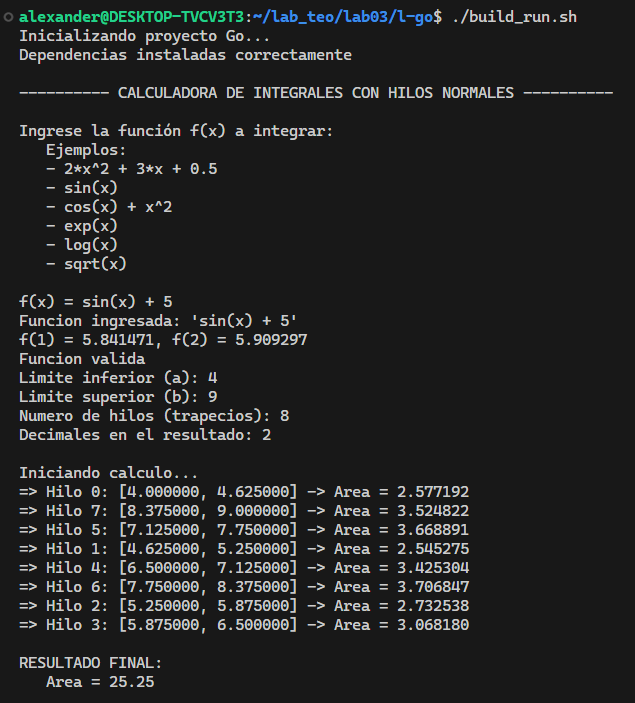
\includegraphics[width=0.8\linewidth]{img/go_prueba_hilo_1.PNG}
    \caption{Prueba de ejecución para la implementación inicial}
    \label{fig:placeholder}
\end{figure}

\textbf{Prueba de ejecución para la primera implementación con Pool de threads en golang}

\begin{figure}[H]
    \centering
    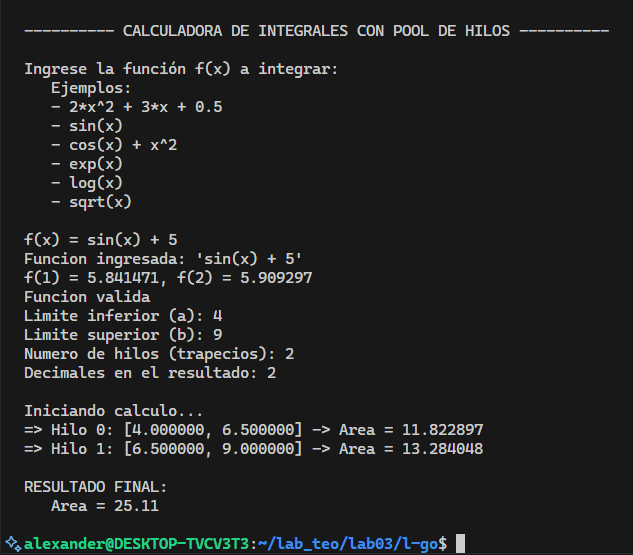
\includegraphics[width=0.8\linewidth]{img/go_prueba_pool_1.PNG}
    \caption{Prueba de ejecución}
    \label{fig:placeholder}
\end{figure}

\textbf{Prueba de ejecución para la primera implementación de java}

\begin{figure}[H]
    \centering
    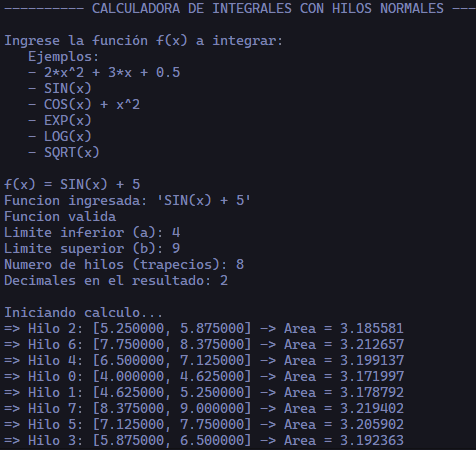
\includegraphics[width=0.8\linewidth]{img/java_prueba_hilo_1.png}
    \caption{Prueba de ejecución para la implementación inicial}
    \label{fig:placeholder}
\end{figure}

\textbf{Prueba de ejecución para la primera implementación con Pool de threads en java}

\begin{figure}[H]
    \centering
    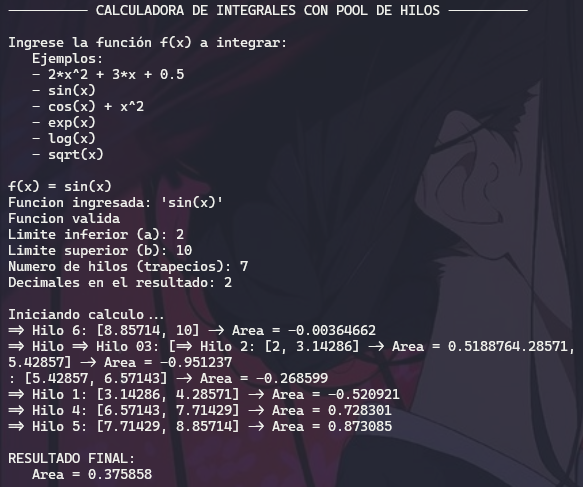
\includegraphics[width=0.8\linewidth]{img/java_prueba_pool_1.png}
    \caption{Prueba de ejecución}
    \label{fig:placeholder}
\end{figure}

\textbf{Prueba de ejecución para la primera implementación de cpp}

\begin{figure}[H]
    \centering
    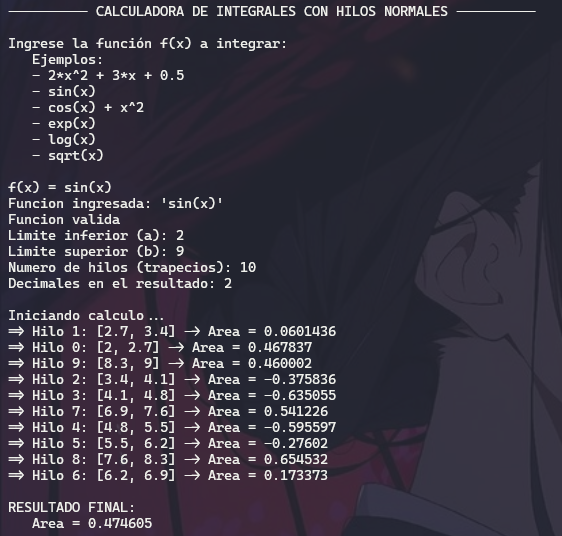
\includegraphics[width=0.8\linewidth]{img/cpp_prueba_hilo_1.png}
    \caption{Prueba de ejecución para la implementación inicial}
    \label{fig:placeholder}
\end{figure}

\textbf{Prueba de ejecución para la primera implementación con Pool de threads en cpp}

\begin{figure}[H]
    \centering
    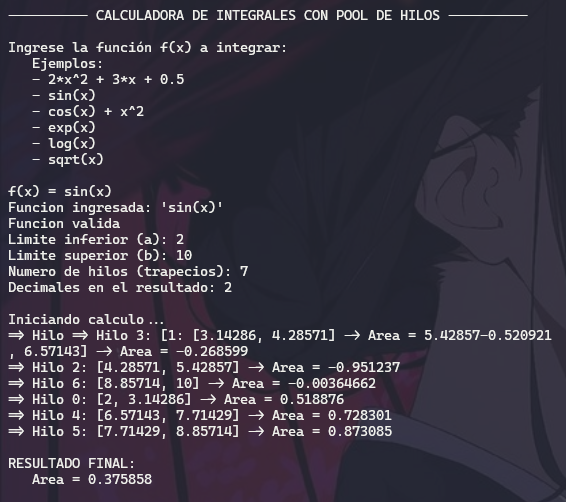
\includegraphics[width=0.8\linewidth]{img/cpp_prueba_pool_1.png}
    \caption{Prueba de ejecución}
    \label{fig:placeholder}
\end{figure}


\subsection {Commits realizados}

\subsubsection {Primer Commit}

\begin{itemize}
    \item Este commit se hizo despues de completar en un 80\% el código de la implementación en c++
    \item Se crearon las clases requeridas, CmakeList para las librerias que se requieren
    \item Una clase main para probar el funcionamiento de las clases implementadas.
\end{itemize}

\begin{figure}[H]
    \centering
    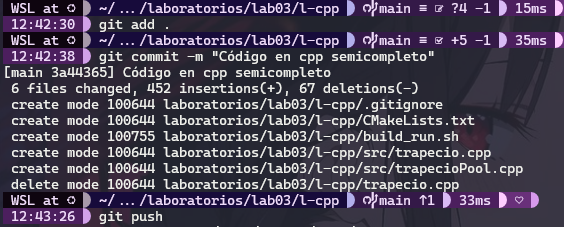
\includegraphics[width=0.8\linewidth]{img/commit01.png}
    \caption{Commit 01}
    \label{fig:placeholder}
\end{figure}


\subsubsection {Segundo Commit}

\begin{itemize}
    \item Este commit se hizo despues terminar la implementación de código para golang, despues de probar el funcionamiento.
\end{itemize}

\begin{figure}[H]
    \centering
    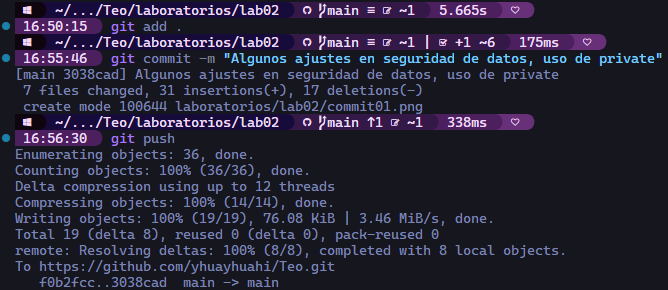
\includegraphics[width=0.8\linewidth]{img/commit02.PNG}
    \caption{Commit 02}
    \label{fig:placeholder}
\end{figure}


\subsubsection {Tercer Commit}

\begin{itemize}
    \item En este commit se completo la implementación del código para java
    \item Se uso Maven como administrador de paquetes
\end{itemize}

\begin{figure}[H]
    \centering
    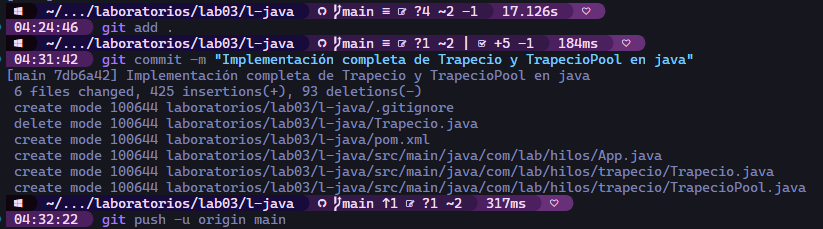
\includegraphics[width=0.8\linewidth]{img/commit03.png}
    \caption{Commit 03}
    \label{fig:placeholder}
\end{figure}


\subsection {Estructura del laboratorio}

A continuación se muestra la estructura de archivos y carpetas del laboratorio realizado:
Claramente los archivos de compilación de Java y otros que se pudieron generar no se subieron al repositorio.


\begin{figure}[H]
    \centering
    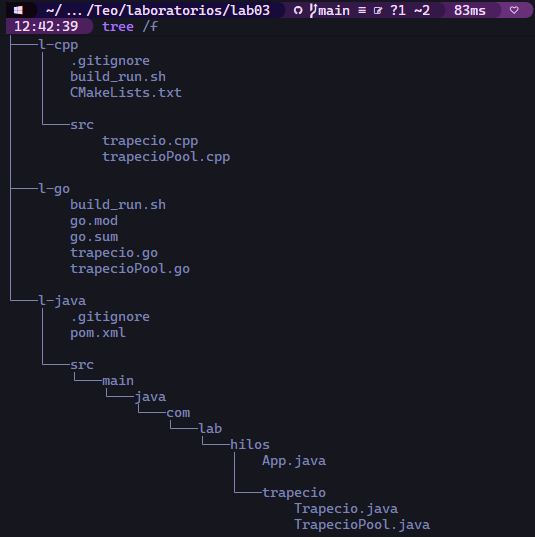
\includegraphics[width=0.8\linewidth]{img/estructura.png}
    \caption{Estructura de laboratorio}
    \label{fig:placeholder}
\end{figure}



\section{Cuestionario}

\subsection{¿Cuál de los LP posee ventajas para programar paralelamente?}

\begin{itemize}
    \item Java y Go poseen ventajas para programar paralelamente debido a que soportan concurrencia y paralelismo de manera nativa. En Java, se tiene la API de concurrencia y los hilos, mientras que en Go tiene goroutines y canales, lo que facilita la programación concurrente.
\end{itemize}


\subsection{¿Para cada lenguaje elabore una tabla cuando usa Pool de Treads?}

\begin{itemize}
    \item \textbf{Java}: Utiliza Executors para manejar pools de hilos.
    \item \textbf{Cpp}: Puede usar bibliotecas como ThreadPool para implementar pools de hilos.
    \item \textbf{Golang}: Utiliza goroutines y canales, pero no tiene un pool de hilos tradicional.
\end{itemize}




